\documentclass[letterpaper, 12pt]{article}
\usepackage{amssymb,amsmath,amsthm,amsbsy}
\usepackage{setspace}
\setstretch{1.7}
\usepackage{geometry}
\geometry{letterpaper, textwidth=6.5in}
\usepackage[colorlinks = true, citecolor=blue, linkcolor=blue, urlcolor=blue]{hyperref}

\usepackage{natbib}
%\usepackage[strings]{underscore}

\usepackage{lscape,graphicx,caption,subcaption,booktabs}
\usepackage{outlines}
\usepackage{enumitem}
\usepackage{afterpage}

\makeatletter
\title{\vspace*{-2em}Democracy in America? \\ Partisanship, Polarization, and the Robustness of Support for Democracy in the United States\thanks{We would like to thank Jacob Hacker, David Hendry, Greg Huber, Steven Levitsky, David Mayhew, Nolan McCarty, Adam Przeworski, Arturas Rozenas, Daniel Treisman, Bonnie Weir, and audiences at APSA, EPSA, Boston University, Caltech, Columbia, Georgetown, Harvard, IAS Toulouse, Peking University, Technical University of Munich, Texas A\&M, UC Berkeley, UT Austin, Vanderbilt, and Yale for helpful comments and conversations and Isaiah Affron and Lily Engbith for research assistance. This project was supported by the Institution for Social and Policy Studies and the Whitney and Betty MacMillan Center for International and Area Studies, both at Yale University.}}

\author{Matthew H. Graham\thanks{Ph.D. Candidate, Department of Political Science, Yale University, \href{email:matthew.graham@yale.edu}{matthew.graham@yale.edu}.} \hspace{1mm} and Milan W. Svolik\thanks{Professor, Department of Political Science, Yale University, \href{email:milan.svolik@yale.edu}{milan.svolik@yale.edu}.}}
\date{First draft: March 2018, current version: December 2019}

\begin{document}

\newgeometry{top=1in, bottom=1in}
\begin{titlepage}
\maketitle
\thispagestyle{empty}

\begin{abstract}
\singlespacing
Is support for democracy in the United States robust enough to deter undemocratic behavior by elected politicians? We develop a model of the public as a democratic check and evaluate it using two empirical strategies: an original, nationally representative candidate-choice experiment in which some politicians take positions that violate key democratic principles, and a natural experiment that occurred during Montana's 2017 special election for the U.S. House. Our research design allows us to infer Americans' willingness to trade-off democratic principles for other valid but potentially conflicting considerations such as political ideology, partisan loyalty, and policy preferences. We find the U.S. public's viability as a democratic check to be strikingly limited: only a small fraction of Americans prioritize democratic principles in their electoral choices and their tendency to do so is decreasing in several measures of polarization, including the strength of partisanship, policy extremism, and candidate platform divergence. Our findings echo classic arguments about the importance of political moderation and cross-cutting cleavages for democratic stability and highlight the dangers that polarization represents for democracy.
\end{abstract}

\end{titlepage}

\begin{raggedright}
\restoregeometry
\setlength{\topmargin}{-0.5in}
\setlength{\textheight}{8.5in}
\parindent=0.25in

\begin{flushright}
\textit{``It is the function of public opinion to check the use of force in a crisis,\\ so that men, driven to make terms, may live and let live.''}\\
Walter Lippmann, \emph{The Phantom Public} (1925, 64)
\end{flushright}

\section{Introduction}

``It is nearly impossible to find an American who says that he is opposed to democracy or favors some alternative\dots On the contrary, nearly everyone professes to believe that democracy is the best form of government.'' This is how Robert A. Dahl, writing in 1966, summarized contemporary evidence for the support for democracy in the United States \citep[40]{Dahl1966}. It remains conventional wisdom to this day. Research that traces its intellectual origins to Tocqueville's \emph{Democracy in America} finds that the United States consistently exhibits some of the highest levels of support for democracy in the world \citep{Almond1963, Inglehart2010, Norris2011}.

We show that this conventional wisdom rests on fragile foundations. Rather than asking about support for democracy directly, we adopt an approach that infers Americans' commitment to democratic principles from their choices of candidates in hypothetical election scenarios. Each candidate is experimentally assigned attributes and platforms that approximate real-world elections and, crucially, may endorse positions that violate core democratic principles, including free and fair elections, civil liberties, and checks and balances. In this framework, voters ``support democracy'' not when they say so, but rather when their choices \emph{reveal} a preference for democratic principles over other valid but potentially conflicting considerations such as political ideology, partisan loyalty, or policy preferences.

This research design builds on the observation that elections represent a fundamental instrument of democratic self-defense: Especially in advanced democracies, voters have the opportunity to stop politicians whose positions violate democratic principles by defeating them at the polls. We argue that a key obstacle to the viability of such a democratic check is partisan, ideological, and policy-based polarization. Electoral competition often confronts voters with a choice between two valid but potentially conflicting considerations: partisan interests and democratic principles. Polarization raises the stakes of elections and in turn the price of prioritizing democratic principles over partisan interests. When faced with the choice between a co-partisan candidate whose positions violate democratic principles and a candidate who complies with democratic principles but is otherwise unappealing, a significant fraction of voters may sacrifice democratic principles to elect a candidate who champions their party or interests. In a sharply polarized electorate, even pro-democratically minded voters may act as partisans first and democrats only second.

In the next section, we formalize these intuitions and develop a model of the public as a democratic check. Building on \citet{Svolik2019}, we extend the classic, spatial framework for electoral competition to account for candidates who may hold positions that undermine democratic principles. The latter are conceptualized as negative valence attributes: while voters may differ over policy, ideology, or partisanship, they agree that electoral competition should be democratic and prefer candidates who comply with key democratic principles. This framework yields a number of predictions about the consequences of polarization for an electorate's resilience to undemocratic candidates: i) voters who hold extreme or intense policy preferences will be willing to sacrifice democratic principles at higher rates than centrist and moderate voters, ii) electorates that are polarized or lack cross-cutting cleavages will be less punishing of candidates that undermine democratic principles, and iii) candidate platform polarization will be detrimental to democracy independent of voter polarization. Our model thus provides microfoundations for classic arguments about the importance of political moderation and cross-cutting cleavages for democratic stability \citep{Dahl1956,Lipset1960}.

This framework guides the design and analysis of our candidate-choice experiment as well as a natural experiment that occurred during Montana's 2017 special election for the U.S. House. The following is a summary of our experimental findings:
\begin{description}[style=unboxed,leftmargin=0em,itemsep=0em]
\item[1. Americans value democracy, but not much:] A candidate who considers adopting an undemocratic position can expect to be punished by losing only about 11.7\% of his overall vote share. When we restrict attention to candidate-choice scenarios with combinations of partisanship and policies that we typically see in real-world elections, this punishment drops to 3.5\%.
\item[2. Support for democracy is highly elastic:] When the price of voting for a more democratic candidate is that candidate's greater distance from the voter in terms of her preferred policies, even the most centrist voters are willing to tolerate at most a 10-15\% increase in such a distance.
\item[3. Centrists are a pro-democratic force:] ``Centrist'' voters who see small policy differences between candidates punish undemocratic behavior at four times the rate of ``extremist'' voters who give a decisive advantage to one candidate or the other.
\item[4. Most voters are partisans first and democrats only second:] Only about 13.1\% of our respondents are willing to defect from a co-partisan candidate for violating democratic principles when the price of doing so is voting against their own party. Only independents and partisan ``leaners'' support more democratic candidates enough to defeat undemocratic ones regardless of their partisan affiliation.
\item[5. Supporters of both parties employ a partisan ``double standard:''] Respondents who identify as Republican are more willing to punish undemocratic behavior by Democratic Party than Republican Party candidates and vice versa. These effects are about equal among both Democrat and Republican respondents.
\item[6. Platform polarization is bad for democracy:] The larger the difference between the candidates' policy platforms, the weaker is the punishment for undemocratic behavior.
\item[7. Sensitivity to the menu of manipulation varies:] Voters are most punishing of undemocratic positions that undermine the free press and the rule of law; they are least punishing of restrictions on the freedom of assembly and executive aggrandizement. Nonetheless, when we benchmark these against extramarital affairs and underpaying of taxes -- two negative valence attributes unrelated to democracy -- we find that voters punish the latter \emph{more} severely than they punish violations of democratic principles.
\item[8. Americans have a solid understanding of what democracy is and what it is not:] The vast majority of our respondents correctly distinguish real-world undemocratic practices -- including those endorsed by our experimental candidates -- from those that are consistent with democratic principles.
\end{description}

After examining these findings non-parametrically, we take advantage of the close connection between the design of our candidate-choice experiment and our theoretical framework and adopt a structural approach. This approach allows us to parsimoniously summarize the variation in our respondents' candidate choices using a few theoretically-grounded parameters, including the weight that voters place on democracy relative to party and policy. We estimate this weight at 18\% and find that candidates' democracy positions, economic and social policy platforms, and partisan affiliation jointly account for 80\% of the systematic variation in voters' candidate choices. We also ``price'' democracy in terms of the candidate characteristics voters are willing to forgo to punish candidates who violate democratic principles. We find that this price corresponds to about half the difference between our respondents' favorite and least favorite policy positions. We then extend our theoretical model to account for our experimental findings about a partisan double standard in the punishment of candidates who violate democratic principles. We estimate a 48.4\% co-partisan bias, implying that Americans are neither fully principled nor purely instrumental in their support for democracy.

The last portion of our analysis moves from hypothetical election scenarios to a real-world election: a natural experiment that occurred during the 2017 special election for Montana's only seat in the U.S. House of Representatives. On the eve of the election, one of the two major candidates assaulted a journalist, which we interpret as a negative public signal about his respect for a free press, or at a minimum, an undesirable valence attribute. Crucially, only election day voters saw this signal before they voted; absentee voters, who in Montana make up a majority of registered voters, had already cast their ballots. This allows us to adopt a difference-in-differences empirical strategy that compares precinct-level vote shifts between absentee and election day voters to infer their willingness to punish the assault. Our findings are consistent with both our theoretical expectations and experimental results. We find that only moderate precincts punished the assault on the journalist by voting across party lines. In heavily partisan precincts, partisan loyalty trumped valence considerations.

Our findings about the robustness of support for democracy in the United States contribute to a number of debates in comparative and American politics. Most immediately, our paper joins a growing body of work that has, in the wake of the 2016 presidential election, begun to reassess our knowledge about democratic stability in the United States\footnote{See especially \citet{Carey2018}, \citet{HuqGinsburg2017}, \citet{KaufmanHaggardForthcoming}, \citet{LiebermanMettlerPepinskyEtAlForthcoming}, \citet{Miller2017}, and \citet{Przeworski2019}.} and other advanced democracies.\footnote{See \citet{BecherBrouard2019}, \citet{Foa2017}, and \citet{Voeten2017}.} Theoretically, our arguments parallel \citet{Levitsky2018}, who also highlight the dangers that polarization represents for democratic stability. While their analysis focuses primarily on how polarization weakens the often informal norms that regulate interactions among political elites, our emphasis is on how polarization undermines the public's capacity to punish politicians for subverting the democratic process.

Our empirical methodology and substantive focus are closest to \citet{Carey2018a}, who also employ a candidate-choice experiment to study the commitment to democratic principles among the American public. They too report that while voters do punish candidates whose positions violate democratic principles, the magnitude of that punishment may be overshadowed by other political considerations -- most notably partisanship. As we discuss in the conclusion, these findings suggest that conventional, direct-questioning measures of support for democracy may be flawed because they fail to account for voters' willingness to trade off democratic principles for partisan interests. In turn, our existing knowledge about the support for democracy in the United States and other advanced democracies is of limited utility when it comes to answering a key question: When can we realistically expect the public to check the authoritarian temptations of elected politicians?

Our theoretical framework helps us to address this question by proposing a new perspective on democratic stability: democracy is ``self-enforcing'' when politicians anticipate that, were they to behave undemocratically, their own supporters would punish them by voting for a competitor in large enough numbers to bring about their defeat. We explain why this electoral check may fail in polarized societies and even among voters who value democracy for its own sake: in sharply divided societies, voters put partisan ends above democratic principles.\footnote{The trade-off between partisan interests and democratic principles can be seen as a special case of a more general trade-off between partisan and valence considerations \citep{AshworthMesquita2009}. Such an interpretation of our findings echoes \citet{Eggers2014a} who finds that voters punished politicians implicated in the 2009 U.K. expenses scandal less severely when the electoral stakes in their district were higher.} The microfoundations that we develop thus combine insights from two lines of classic democratization research. The first views intense political cleavages as a threat to democratic stability \citep{Dahl1956,Lipset1960}; the second asks that explanations of democratic stability be explicit about the incentives of key actors to comply with the rules of democratic politics \citep{przew91,weingast97}. More broadly, we contribute to comparative politics research on democratic backsliding \citep{Gandhi2018,Haggard2016,LuoPrzeworski2018,Nalepa2018,WaldnerLust2018}.

Jointly, our theoretical framework and empirical findings suggest an explanation for the puzzling persistence in the United States of a number of deficiencies in the democratic process, especially at the state and local level. Most frequent among these are gerrymandering \citep{Chen2013,ChoLiu2016} and voter suppression \citep{Grimmer2018}. Our model implies that elected officials' incentives to comply with key democratic principles critically depend on the public's willingness to sanction those who violate them or neglect their enforcement.\footnote{\citet{Clark2009} sees a similar role for public opinion in his analysis of court curbing.} Yet our empirical analysis reveals that this check is at best limited in magnitude and subject to a partisan double standard. As we discuss in the conclusion, our findings imply that public officials may be effectively insulated from electoral sanction in states and districts where one party enjoys a significant electoral advantage.

Analytically as well as empirically, we examine the pernicious consequences of a number of distinct conceptions of polarization. At the level of individual voters, polarization may characterize voters who hold either extreme or intense preferences. At the level of the electorate, polarization may correspond to either a U-shaped distribution of voter preferences or one with a high correlation of preferences across issues or between issue areas and partisan affiliation. At the level of the candidates, polarization can be conceived of as corresponding to a large distance between candidate platforms. These distinct conceptions of polarization are rarely examined within a single theoretical framework. Our analysis demonstrates that each kind of polarization independently undermines the electorate's resilience to undemocratic candidates.

This comprehensive examination of the relationship between polarization and democratic stability contributes to a large research agenda that studies elite and mass polarization in the United States. Whereas most research on mass polarization focuses on characterizing its nature and origins \citep{Abramowitz2008,Fiorina2008,McCarty2008,Iyengar2018}, our focus is on a political consequence that this literature has yet to examine.\footnote{Because our primary focus is on mass polarization, we do not discuss research on polarization in Congress. For a review of this literature, see \citet{BarberMcCarty2015}.} To our knowledge, our study is the first to examine what is possibly the most concerning consequence of increasing polarization in the United States: its potential to undermine the public's ability to check the undemocratic temptations of elected politicians.

\section{A Model of the Public as a Democratic Check}
\label{sec: model}

Consider a model in which voters' preferences over two kinds of candidate attributes determine their electoral choices: i) positional issues, including candidates' policy positions, ideology, and partisan affiliation, and ii) candidates' compliance with key democratic principles. Building on \citet{Svolik2019}, we conceive of the latter as a valence issue: while voters may differ over policy, ideology, or partisanship, they all prefer candidates whose positions comply with key tenets of democratic electoral competition.

Formally, voter $i$'s payoff from candidate $j$ is
\begin{equation}
\label{eq: utility}
u_i(X_j, M_j) = -\sum\limits_{k=1}^K \alpha_k (x_{ik} - x_{jk})^2 - \delta M_j \, ,
\end{equation}
where, for each of $K$ issues, $x_{ik}$ is voter $i$'s favorite position on issue $k$, $x_{jk}$ is candidate $j$'s platform on issue $k$, and $\alpha_k$ is the weight that $i$ attaches to that issue. Meanwhile, $M_j$ is candidate $j$'s democracy position where $M$ is increasing in how \emph{un}democratic $j$'s platform is ($M$ stands for ``manipulation''). The term $\delta$ is the weight that voters attach to fair democratic competition -- in effect, the intensity of their support for democracy.

This model yields several predictions that we evaluate throughout the paper. First, voters who hold intense or extreme policy preferences are willing to tolerate undemocratic behavior by their favored candidate. To see the intuition behind these predictions, suppose there is only a single policy issue $k$. Then $i$ votes for candidate~1 as long as
\begin{equation}
\label{eq: ineq}
x_{ik} \ge \frac{x_{1k} + x_{2k}}{2} + \frac{\delta(M_1- M_2)}{2 \alpha_k (x_{1k} - x_{2k})} \, \quad \text{for} \quad x_{1k} > x_{2k},
\end{equation}
where we are assuming that candidate~1's policy platform is to the right of candidate~2's platform.

Call the voter whose ideal policy $x_{ik}$ barely satisfies the inequality in \eqref{eq: ineq} the \emph{swing voter} $x_{s}^{j}$. Note that the first term on the right-hand side of this inequality is the midpoint between the two candidates' policy platforms, separating the electorate into those who are policy-wise closer to candidate~1 and those who are closer to candidate~2. The swing voter $x_{s}^{j}$ is located either to the right or the left of this midpoint, depending on which of the two candidates adopts an undemocratic position,
\begin{equation}
\label{eq: demfirst}
x_{s}^1, x_{s}^2 = \frac{x_{1k} + x_{2k}}{2} \pm \frac{\delta}{2 \alpha_k (x_{1k} - x_{2k})} \, .
\end{equation}

When candidate~1 adopts an undemocratic position ($M_1=1$, $M_2=0$), the swing voter $x_{s}^{1}$ is located to the right of the midpoint $\frac{x_{1k} + x_{2k}}{2}$. Voters to the right of the midpoint but to the left of $x_{s}^1$ favor candidate~1 based on their policy preferences, yet are sufficiently put off by his undemocratic position that they vote for candidate~2 instead. By contrast, voters whose policy preferences are extreme (large $x_{ik}$) or intense (a large $\alpha_k$) enough to be to the right of $x_{s}^1$ are willing to tolerate candidate~1's undemocratic position as their concern for democracy is outweighed by their proximity to his policies. The converse holds when candidate~2 adopts an undemocratic platform.

The segment between the two swing voters is related to another set of empirical predictions. It delineates the set of voters who always vote for the more democratic of the two candidates. We may therefore refer to this portion of the electorate as ``democracy first'' voters, as opposed to ``policy first'' voters. The fraction of voters in each category depends on both the length of this segment and the distribution of voters’ ideal points. Its length $\frac{\delta}{\alpha_k (x_{1k} - x_{2k})}$ is increasing in the support for democracy $\delta$; it is decreasing in the policy weight $\alpha_k$ and the distance between the candidates' platforms $(x_{1k} - x_{2k})$.

Meanwhile, the more polarized (U-shaped) the distribution of voters' ideal policies is, the smaller the fraction of democracy first voters. The consequences of voter polarization are amplified when voters' preferences over the $K$ policy issues correlate: when a voter's extreme position on one issue correlates with her extreme position on another, her preference for the more proximate candidate will compound across the two issues rather than cancel out.

The primary purpose of this framework is to guide the design of our candidate-choice experiment and the analysis of our data. This has shaped our theoretical analysis in two ways. First, we have intentionally treated the candidates' policy platforms and democracy positions as exogenous, as these will be randomly assigned in the candidate-choice experiment that we introduce in the next section.\footnote{For a model with endogenous policy and democracy positions, see \citet{Svolik2019}.}

Second, in order to explicitly characterize the model's implications for our analysis of the candidate-choice experiment, we introduce a stochastic structure into the deterministic formulation of the voters' payoff in \eqref{eq: utility} and outline its consequences. We follow the classic random utility model of discrete choice and add to voter $i$'s payoff from candidate $j$ an error term $\epsilon_{ij}$,
\begin{equation}
\label{eq: random utility}
u_i(X_j, M_j) = -\sum\limits_{k=1}^K \alpha_k (x_{ik} - x_{jk})^2 - \delta M_j + \epsilon_{ij}\, .
\end{equation}
Assuming that the error terms $\epsilon_{ij}$ are (independently) drawn from type I extreme value distribution implies that the effect of candidate positions on voter $i$'s probability of voting for a candidate can be estimated using the logistic regression.\footnote{This is only one of several plausible stochastic structures; see \citet[476-478, 486-487]{Cameron2005}.} We take advantage of this correspondence between our theoretical framework and the random utility model of discrete choice when we estimate the model's key parameters, including civic virtue $\delta$ and policy weights $\alpha_k$.

Here we highlight the aggregate empirical patterns implied by this stochastic formulation. First, in contrast to the deterministic case, the two swing voters no longer sharply separate ``democracy first'' from ``policy first'' voters. Rather, the segment between the two swing voters now delineates voters who, regardless of their policy proximity to the candidates, vote for the more democratic candidate with a probability greater than one-half. The left panel in Figure \ref{fig: model} illustrates this by plotting a voter's probability of voting for candidate~1 as a function of ideal policies $x_{ik}$ over a single issue $k$.\footnote{Figure \ref{fig: model} is based on parameter values $\alpha_k=8$, $\delta=2$, and $x_{1k}=- x_{2k}=1/5$.} The black solid line plots the case when both candidates adopt a democratic position; the dashed line plots the case when candidate~1 adopts an undemocratic position.

An alternative interpretation of the vertical axis in the left panel of Figure \ref{fig: model} that we employ when analyzing the candidate-choice experiment is that it corresponds to the fraction of voters in subgroups along the horizontal axis that support candidate~1. Furthermore, it will often be more practical to use as the horizontal axis the difference in voters' policy proximity to the two candidates rather than voters' ideal points alone. In that case, the intersection of the dashed curve with the .5 horizontal line will, instead of the swing voter $x_{s}^1$, mark the quantity $\frac{\delta}{\alpha_k}$, which we later interpret as voters' value for democracy in terms of issue $k$.


A key quantity that we estimate throughout the paper is the overall fraction of voters who defect from a candidate that adopts an undemocratic position, which we denote by $\Delta$. In effect, $\Delta$ measures the public's ability to serve as a democratic check and results from a combination of two factors: the rate at which voters defect from the undemocratic candidate and the distribution of voters.\footnote{That is, $\Delta = \int_{-\infty}^{\infty} \left(\frac{1}{1+e^{-D}}-\frac{1}{1+e^{-(D - \delta M_1)}}\right) dF(x_i)$, where $F(x_i)$ is the distribution of voters and $D=\sum\limits_{k=1}^K \alpha_k (x_{ik} - x_{2k})^2-\sum\limits_{k=1}^K \alpha_k (x_{ik} - x_{1k})^2$.} The right panel in Figure \ref{fig: model} plots the former. It shows that while centrists will in general defect from undemocratic candidates at higher rates than extremists, the maximum defection rate (marked by $x^1_{\Delta}$) will be located to the right of the midpoint $\frac{x_{1k} + x_{2k}}{2}$ but to the left of the swing voter $x_{s}^1$. Intuitively, it is voters who would otherwise narrowly break in favor of candidate~1 that abandon him at the highest rates once he adopts an undemocratic position.

%\begin{landscape}
\begin{figure}[t]
\centering
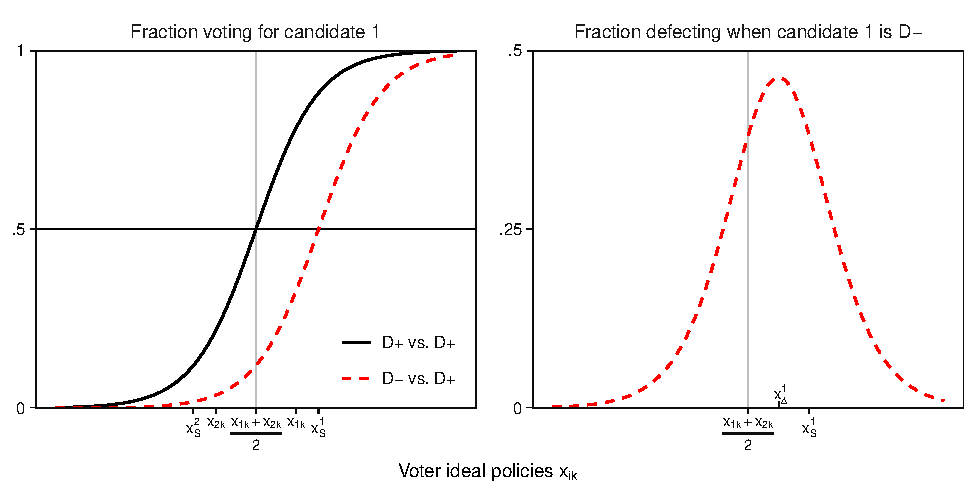
\includegraphics{figures/fig1_manual.pdf}

\caption{Model predictions: The fraction voting for candidate~1 (left) and the decline in the less democratic candidate's vote share (right)}
\label{fig: model}
\end{figure}
%\end{landscape}


To recapitulate, this theoretical framework yields five predictions about the relationship between a number of distinct conceptions of polarization and a decline in the public's ability to serve as a democratic check, which we denote by $\Delta \downarrow$:\footnote{See the appendix for a formal statement and proofs of these predictions.}
\begin{description}[style=unboxed,leftmargin=1em,itemsep=0em]
\item[1. Centrists are a pro-democratic force:] $\Delta \downarrow$ for voters whose policy preferences are more \emph{extreme} relative to the candidates' platforms ($x_{ik}$ far from the midpoint $\frac{x_{1k} + x_{2k}}{2}$);
\item[2. Moderation is good for democracy:] $\Delta \downarrow$ for voters who hold more \emph{intense} policy preferences (a large $\alpha_k$);
\item[3. Voter polarization is bad for democracy:] $\Delta \downarrow$ as the \emph{distribution} of voters' ideal policies becomes more U-shaped (polarized) as opposed to inverse-U shaped (centrist);
\item[4. Candidate polarization is bad for democracy:] $\Delta \downarrow$ as the \emph{distance} between candidate platforms increases (large $|x_{1k} - x_{2k}|$);
\item[5. Cross-cutting cleavages are good for democracy:] $\Delta \downarrow$ when voter preferences over the $K$ distinct issues are \emph{aligned} as opposed to \emph{cross-cutting} with respect to candidates platforms.
\end{description}

\section{The Candidate-Choice Experiment}
\label{sec: conjoint}

Our candidate-choice experiment investigates a key mechanism underlying the above predictions: even voters who value democratic principles may trade off those principles for partisan ends when confronted with a choice between the two. By asking respondents to choose between two candidates in an election, the experiment examines this mechanism at the same level at which it is hypothesized to operate -- that of the individual voter. Moreover, because it entails one of the most essential and familiar actions that democratic citizens perform -- voting -- the experiment allows us to study our respondents' willingness to trade off democratic principles for partisan interests without alerting them to it.

In the candidate-choice experiment, respondents made a series of 16 choices, each between two candidates for a state legislature. The candidates were described by experimentally manipulated attributes typically seen in real-world elections: age, gender, race, profession, years of experience, partisan affiliation, two policy platforms, and a ``democracy'' position. This last attribute is the focus of our analysis; we therefore describe its design and assignment below. We introduce most of the remaining attributes throughout the paper. The appendix describes our design in detail and presents an example of a candidate-choice scenario as seen by our respondents.

Each candidate was assigned a democracy position that was either ``undemocratic'' -- an action or statement by the candidate that violates a key democratic principle -- or a democratically neutral, ``generic'' position. The undemocratic positions are listed in Table~\ref{tab: treatments} and labelled $D^-$. There, [own party] refers to a candidate's randomly assigned political party (Democrat or Republican); [opposite party] denotes the complement. For instance, one possible realization of item 4 reads ``Said the Republican governor should ignore unfavorable court rulings by Democrat-appointed judges.''

{
\def\sep{0.3em}
\def\ssep{-0.3em}
\def\fns{\footnotesize}
\def\onepc{$^{\ast\ast\ast}$} \def\fivepc{$^{\ast\ast}$}
\def\tenpc{$^{\ast}$}
\def\legend{\multicolumn{3}{l}{\footnotesize{Significance levels
:\hspace{1em} $\dag$ : 10\% \hspace{1em}
$\ast$ : 5\% \hspace{1em} $\ast\ast$ : 1\% \normalsize}}}

\begin{table}[t!]\centering
\caption{Undemocratic positions endorsed by candidates assigned to the $D^-$ treatment condition}
\label{tab: treatments}
\vspace{2mm}
\small
\begin{tabular}{l l l}

\toprule

\boldmath${D^-}$ & \textbf{Undemocratic Position} & \textbf{Democratic Principle} \\

\toprule

1a & Supported a redistricting plan that gives [own party]s & Electoral fairness \\
& 2 extra seats despite a decline in the polls. & \\[\sep]
1b & Supported a redistricting plan that gives [own party]s & Electoral fairness \\
& 10 extra seats despite a decline in the polls. & \\[\sep]
2 & Supported a proposal to reduce the number of polling & Electoral fairness \\
& stations in areas that support [opposite party]s. & \\[\sep]
3 & Said the [own party] governor should rule by executive & Checks and balances \\
& order if [opposite party] legislators don't cooperate. & \\[\sep]
4 & Said the [own party] governor should ignore unfavorable & Checks and balances \\
& court rulings by [opposite party]-appointed judges. & \\[\sep]
5 & Said the [own party] governor should prosecute journalists & Civil liberties \\
& who accuse him of misconduct without revealing sources. & \\[\sep]
6a & Said the [own party] governor should ban far-left & Civil liberties \\
& group rallies in the state capital. & \\[\sep]
6b & Said the [own party] governor should ban far-right & Civil liberties \\
& group rallies in the state capital. & \\[\sep]
\bottomrule

\end{tabular}

\end{table}
}

In designing these undemocratic positions, we employed the following criteria:
\begin{description}[style=unboxed,leftmargin=0em,itemsep=0em]
\item [Conceptual validity:] The undemocratic positions capture violations of key democratic principles. Following classic scholarship on democratization \citep{dahl71}, this includes measures that undermine electoral fairness (items 1a, 1b, and 2 in Table~\ref{tab: treatments}), checks and balances (items 3 and 4), and civil liberties (items 5, 6a, and 6b).

We also verify that our respondents indeed see the positions in Table~\ref{tab: treatments} as undemocratic. One to three weeks before the candidate-choice experiment, each respondent was asked to evaluate a battery of both democratic and undemocratic practices, including the practices that would later appear as our $D^-$ treatments. As we document in the appendix, the vast majority of our respondents correctly rated the $D^-$ treatments as ``undemocratic.’’

\item [Contextual realism and partisan balance:] The undemocratic positions approximate practices that have been used by politicians to subvert the democratic process in the United States and can be plausibly adopted by both major parties. Accordingly, the undemocratic positions are situated at the state level, where most attempts to subvert the democratic process for partisan gain in the United States occur and have historically been attempted by both major parties. The appendix provides real-world examples of each undemocratic position.

\item [Incremental violations:] A key feature of attempts to subvert the democratic process, both in the United States and around the world, is the use of ostensibly legal, incremental, and complementary measures \citep{Levitsky2018,WaldnerLust2018}. This has several consequences. First, such measures must often be implemented by or in conjunction with the executive. This is why some of our undemocratic positions refer to actions that the candidate suggests a co-partisan governor take. Second, because such measures are typically adopted through a constitutionally mandated process, they may undermine democratic principles without violating the law. This applies to items 1a, 1b, and 3. Finally, any single measure may allow for a partisan interpretation according to which it is consistent with some -- often more majoritarian -- conception of democracy or corrects an existing deficiency in the democratic process. For instance, proponents of stricter voter ID laws respond to accusations of voter suppression by claiming that such measures are needed to prevent voter fraud, and proponents of gerrymandering may claim to be correcting an unfair status quo. Jointly and in their political context, however, such measures result in an uneven playing field that favors their proponents \citep{Levitsky2010,Schedler2002}.

\item [Neutral presentation:] The undemocratic positions were presented in a manner that avoids conspicuousness or normatively leading language. To prevent candidates not assigned to hold an undemocratic position from appearing visually conspicuous, each was assigned one of seven democratically neutral, ``generic'' positions. For instance, one read: ``Served on a committee that establishes the state legislature's schedule for each session;'' we list the remaining six in the appendix. The content and length of such generic positions were designed to balance the cognitive effort required to distinguish a candidate who endorsed an undemocratic position from one that did not.\footnote{For the same reason, we randomized the order in which candidates' democracy and policy positions were listed.} The wording of our undemocratic positions also avoids negative connotations or normatively leading language. For instance, positions 1a, 1b, and 2 describe gerrymandering and voter suppression, respectively, but we intentionally avoided employing those terms. Put simply, we want respondents to decide for themselves whether or not a position violates a democratic principle.
\end{description}

In the experiment, each respondent made 16 distinct candidate choices of which 11 were based on the following experimental design.\footnote{The remaining five scenarios were designed to provide extensions and robustness checks of our core design. We discuss them in the appendix.} In four randomly chosen scenarios, both candidates adopted one of the democratically neutral, ``generic'' positions. Throughout, we treat these as our control scenarios and label them $D^+ \text{ vs. } D^+$. In seven randomly chosen scenarios, one of the candidates adopted an undemocratic position while the other held a neutral position. We refer to these as our treatment scenarios and label them $D^- \text{ vs. } D^+$. Whether the undemocratic position was held by the candidate visually presented on the left or right was random. To simplify the presentation of our findings, we reshape our data so that candidate~2 always holds a neutral position ($D^+$) and, depending on the experimental condition, candidate~1 varies between $D^+$ and $D^-$.

The candidate-choice experiment was embedded in a nationally representative survey of American voters that took place in August-September 2018.\footnote{The first wave, which asked questions about partisanship, policy preferences, and support for democracy, took place on August 28-29, 2018. The primary focus of the second wave, which took place between September 4-25, 2018, was the candidate-choice experiment. Lucid fielded the survey. A pilot survey was fielded on Amazon Mechanical Turk in March 2018. The appendix benchmarks our sample against demographic data from the US Census Bureau and partisan and attitudinal questions from the 2016 American National Election Study.} The 1,691 respondents made a total of 21,604 candidate choices.

%\clearpage

\subsection{Democratic Principles versus Policy Preferences}
\label{sec: policy}

We begin our analysis of the candidate-choice experiment by examining Americans' willingness to trade off democratic principles for their preferred policies. Each candidate proposed a platform in one economic and one social policy area. Economic policies concerned either state income taxes or state funding for local education; social policies concerned either immigration or marijuana's legal status. These policy areas were randomly assigned but identical across the two candidates. Within each policy area, candidates could adopt one of four platforms, ranging from extreme liberal to extreme conservative. The appendix lists all 16 policy platforms and justifies their selection.

One to three weeks before being presented with the candidate-choice scenarios, respondents rated each of the 16 policy platforms on a 0-100 proximity scale. This allows us to identify each respondent's ideal policy across the four areas and, following our theoretical framework, to compute the squared distance between a respondent's ideal policy and the two candidates' platforms for each of the candidate-choice scenarios that the respondents faced.\footnote{That is, the 0-100 proximity scale is a measure of $x_{ik}-x_{jk}$. For each candidate-choice scenario, this allows us to compute the squared distance $\sum\limits_{k=1}^2  \alpha_k (x_{ik} - x_{jk})^2$ between each respondent's ideal policies and both candidates' platforms, and in turn, candidate 1's policy proximity advantage $D=\sum\limits_{k=1}^2  \alpha_k (x_{ik} - x_{2k})^2-\sum\limits_{k=1}^2  \alpha_k (x_{ik} - x_{1k})^2$.} The results that follow are robust to a range of alternative measures of policy proximity between respondents and candidates and account for the possibility that voters' policy preferences may be ideologically incoherent \citep{Converse1964}, multidimensional \citep{Treier2009}, or non-separable from partisanship. We present these alternative measures in the appendix.

The left panel in Figure \ref{fig: cand_policy} plots the fraction of respondents voting for candidate~1 as a function of the difference in policy proximity to the respondent between candidate~1 and candidate~2.\footnote{``Voting'' here refers to the respondents' stated preference for one of the two candidates. We distinguish between respondents' candidate preferences and their stated intent to turn out to vote in the appendix and in \citet{GrahamSvolik2019}. We find that the stronger a respondent's preference for a $D^-$ candidate, the more likely she is to abstain.} On the horizontal axis, a value of 0 refers to scenarios when the two candidates are equally proximate to the respondent, a value of $1$ ($-1$) to scenarios when candidate~1 is a full scale closer to (further away from) the respondent than candidate~2 on both policy areas. We treat the $D^+ \text{ vs. } D^+$ scenario (black solid line), when both candidates adopt neutral democracy positions but differ across other attributes, as our control condition; we treat the $D^- \text{ vs. } D^+$ scenario (dashed line) as our treatment condition. Vertical bars denote 95\% confidence intervals.\footnote{Because each respondent made multiple choices, estimates that treat all observations as independent may understate statistical uncertainty. Unless otherwise noted, we compute all standard errors and confidence intervals using the block bootstrap, which accounts for dependence by resampling observations at the level of the respondent \citep[see e.g.][]{Bertrand2004}. } Figure \ref{fig: cand_policy} is thus the policy analogue of Figure \ref{fig: model}.

The $D^+ \text{ vs. } D^+$ control scenario provides an initial plausibility check of our design. Consistent with our spatial framework, the closer candidate~1 is to a respondent's ideal policies relative to candidate~2, the more likely the respondent votes for candidate~1. Specifically, the fraction of respondents voting for candidate~1 increases from 13.0\% when candidate~1 is a full scale less proximate to the respondent than candidate~2 to 87.0\% in the opposite case. Furthermore, when the two candidates are equally proximate to respondents, the latter act accordingly and split for the two about evenly. Put simply, a respondent's proximity to each candidate's policy platform is a strong predictor of her candidate choices.

%\begin{landscape}
\begin{figure}[t]
\centering
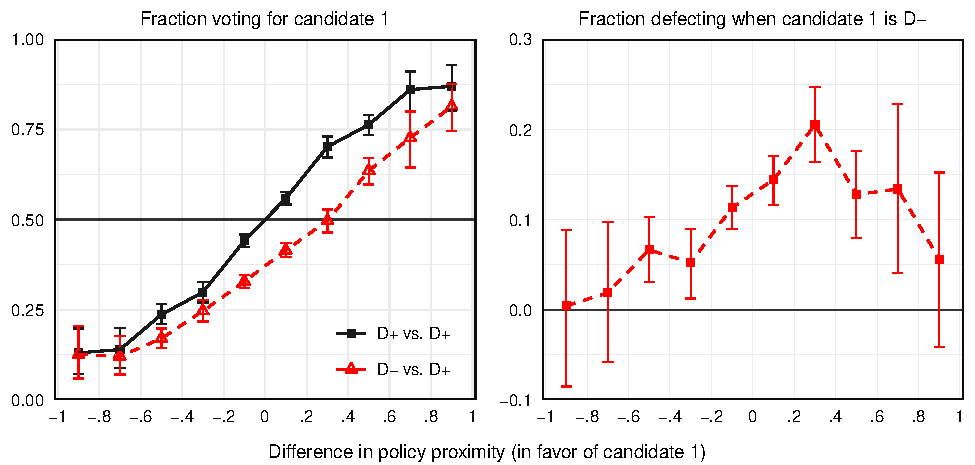
\includegraphics{figures/fig2.pdf}
\caption{Fraction voting for candidate~1 (left) and fraction defecting from the less democratic candidate (right) by the difference between candidates' in policy proximity to the respondent}
\label{fig: cand_policy}
\end{figure}
%\end{landscape}

Figure \ref{fig: cand_policy} also provides an initial estimate of whether and how much Americans value democracy. Because all candidate attributes were randomly assigned, the only systematic difference between our control and treatment conditions is candidate~1's democracy position. We can therefore interpret a decline in the fraction of voters who support candidate~1 in the $D^- \text{ vs. } D^+$ as opposed to the $D^+ \text{ vs. } D^+$ condition as a measure of the public's ability to serve as a democratic check. Considering all candidate-choice scenarios in our experiment, the shift from the $D^+ \text{ vs. } D^+$ to the $D^- \text{ vs. } D^+$ condition decreases candidate~1's vote share from 50.0\% to 38.3\% -- an 11.7\% decline (CI: $10.0, 13.5)$.\footnote{That is, we find both i) that the adoption of a $D^-$ position causes a decline in that candidate's vote share and ii) that a majority of our representative experimental electorate prefers a candidate with a $D^+$ position. As emphasized by \citet{Abramson2019}, finding i) does not necessarily imply ii).} Put differently, just over 10\% of Americans value democracy enough to punish an otherwise favored candidate for violating a democratic principle by voting against him.

Are Americans willing to trade off democratic principles in exchange for more appealing policies? Figure \ref{fig: cand_policy} allows us to address this question by partitioning our experimental electorate into two politically consequential subsets of voters anticipated by our theory: ``democracy first'' and ``policy first'' voters. A majority of the former vote for the more democratic candidate even when doing so goes against their policy interests. These respondents lie in the interval at the center of Figure \ref{fig: cand_policy} between the intersection of the $D^- \text{ vs. } D^+$ line with the 0.5 horizontal axis and its mirror image along that axis. This interval corresponds to the values $(-.3, .3)$ on the horizontal axis and its limits are the empirical counterpart of the two swing voters in Figure \ref{fig: model}. By contrast, voters to the left and right of this interval are ``policy first'' voters: a majority of these supports the more policy-wise proximate candidate, even if that candidate adopts an undemocratic position.

We gain additional insights into the robustness of support for democracy by examining differences in the severity with which respondents punish candidate~1 for adopting an undemocratic platform. The magnitude of this punishment is a combination of two factors: the baseline level of support for candidate~1 in each of the policy proximity subgroups and the rate at which respondents in a subgroup defect from candidate~1 after he adopts an undemocratic position.\footnote{That is, the defection rate is $\rho = \%_{1}(D^+ \text{ vs. } D^+) - \%_{1}(D^- \text{ vs. } D^+)$ where $\%_{1}(T)$ refers to the fraction of respondents voting for candidate~1 in treatment condition $T$.} The right panel in Figure \ref{fig: cand_policy} plots the defection rate. Consistent with our theory, we see that the defection rate is highest among ``bare supporters'' -- respondents who narrowly break in favor of candidate~1 in the $D^+ \text{ vs. } D^+$ scenario -- and declines as we move toward ``policy extremists'' on either side.

These policy-based differences in respondents' willingness to punish undemocratic behavior are consistent with our arguments about the pernicious consequences of polarization for democracy. Our representative sample allows us to simulate counterfactual electorates with increasing levels of policy polarization by varying the ratio of ``policy centrists'' to ``policy extremists.'' As suggested by Figure \ref{fig: cand_policy}, an electorate consisting entirely of ``policy centrists'' -- the middle two bins -- would result in a resounding defeat of a candidate who would adopt an undemocratic platform (12.9\%, CI: 11.1, 15.1). In an electorate consisting entirely of the two most extreme subgroups, undemocratic candidates would only lose 3.0 percentage points of the vote share (CI: -4.1, 11.1), about one-fourth of the penalty among centrists.\footnote{Because the candidates' two policies were independently and randomly assigned, respondents of all types -- those who hold moderate as well as extreme policy preferences -- faced some candidate-choice scenarios in which they were in the position of ``centrists'' and some in which they ``extremists.'' The result is, however, an overall distribution of differences in policy proximity in Figure \ref{fig: cand_policy} that is heavy at the center: about 55\% of scenarios are located on the interval $(-0.1, 0.1)$ and about 78\% on the interval $(-0.3, 0.3)$. To support these claims, the appendix displays the distribution of policy proximity separated by respondents' strength of partisanship and replicates Figure~\ref{fig: cand_policy} using a rank-based measure of respondents' proximity to candidates that, by construction, relies only on within-respondent differences in policy preferences.}


\subsection{Does Partisanship Trump Civic Virtue?}
\label{sec: party}

Are voters willing to put democratic principles ahead of their partisan loyalties? To address this question, consider first only contests between candidates from different parties. Denote by $\text{Rep }D^+ \text{ vs. } \text{Dem }D^+$ the control condition when both candidates adopt a neutral democracy position and by $\text{Rep } D^+ \text{ vs. } \text{Dem } D^-$ and $\text{Rep } D^- \text{ vs. } \text{Dem } D^+$ the treatment conditions in which the Democrat or Republican, respectively, adopts an undemocratic position. Overall, undemocratic candidates are penalized by a loss of 9.9\% (CI: 6.7, 13.0) and 10.9\% (CI: 7.6, 14.0) of voters in the $\text{Rep } D^+ \text{ vs. } \text{Dem } D^-$ and $\text{Rep } D^- \text{ vs. } \text{Dem } D^+$ scenarios, respectively.\footnote{Both penalties imply that a $D^-$ candidate is opposed by a majority respondents, regardless of that candidate's party.} Both effects are statistically different from zero but not statistically different from each other (difference: 1.0\%, CI: -5.3, 3.3). Voters punish undemocratic behavior by both parties and they do so fairly evenly.

\begin{figure}[t]
\centering
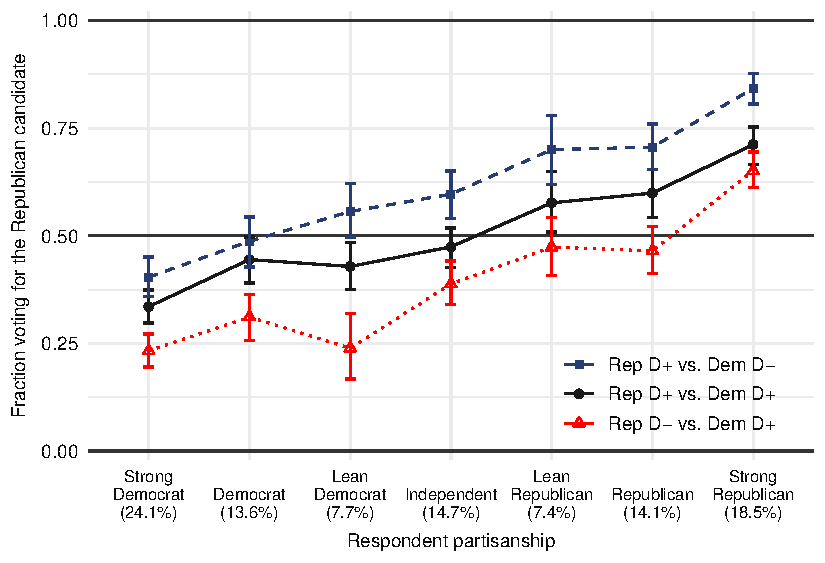
\includegraphics{figures/fig3.pdf}
\caption{Different party contests: Fraction voting for a Republican candidate}
\label{fig: party_diff}
\end{figure}

Are Americans willing to vote across party lines to punish a candidate for adopting an undemocratic position? 63.1\% of our respondents support their own party in the control condition; this number declines to 54.8\% when a respondent's co-partisan adopts an undemocratic position (-8.3\%, CI: 5.0, 11.6). Put differently, only 13.1\% of our respondents are willing to punish a co-partisan for violating democratic principles by voting against their own party, leaving him with a majority support even after he adopts an undemocratic position.\footnote{That is, among respondents who support their own party in the control condition, the treatment effect was 13.1\% of the baseline, $(63.05-54.76)/63.05$. Among respondents who crossed party lines in the control condition, defection is higher: an undemocratic out-partisan's vote share declines from 37.0\% to 24.4\% (-12.6\%, CI: 9.4, 15.9), which is 34.1\% of the baseline, $(36.95 - 24.36)/36.95$.}

Figure \ref{fig: party_diff} yields further insight into how our respondents' willingness to punish undemocratic candidates varies by the strength of their partisanship. It plots the fraction of respondents voting for a Republican Party candidate as a function of our respondents' party identification on the conventional 7-point scale, with the two treatment conditions plotted by dashed and dotted lines. As expected, stronger partisans vote for their party in greater proportion in the control condition, with independents breaking about evenly for the two parties. Only independents who lean toward a party defect from an undemocratic co-partisan in large enough numbers to defeat that candidate. By contrast, respondents who identify as a Democrat or Republican only break even. And a majority of strong partisans would rather elect a candidate that violates democratic principles than cross party lines.

\begin{figure}[t]
\centering

\includegraphics{figures/fig4.pdf}
\caption{Different party contests: Fraction defecting from the less democratic candidate by the respondent's partisanship}
\label{fig: party_frac}
\end{figure}

Strong partisans' failure to punish undemocratic candidates from their own party is the result of two forces. First, strong partisans need to defect from undemocratic candidates at higher rates than moderates to compensate for their high baseline support for co-partisan candidates. Second, they do exactly the opposite: compared to other partisan subgroups, strong partisans are more lenient on violations of democratic principles by candidates from their party. Figure \ref{fig: party_frac} shows this by plotting the fraction of respondents that defect from the $D^-$ candidate, conditioning on both the respondent's and the $D^-$ candidate's partisanship. We see that strong partisans are less than half as likely to punish undemocratic candidates from their own party as are respondents who lean toward the opposite party. Put differently, strong partisans are willing to punish their own for violating democratic principles, but they hold candidates from the other party to a much higher standard.

\begin{figure}[t]
\centering

\includegraphics{figures/fig5.pdf}
\caption{Same party contests: Fraction voting for candidate~1 by the respondent's and the $D^-$ candidate's partisanship}
\label{fig: party_same}
\end{figure}

This raises the question of whether contests between candidates from the same party -- that is, primaries rather than general elections -- are the more viable check on candidates who undermine democratic principles. Consistent with our theory, our respondents are more willing to punish undemocratic candidates in same-party than cross-party contests: a candidate who adopts an undemocratic position is penalized by a loss of 13.3\% and 10.4\% of voters, respectively (difference: 2.9\%, CI: 0.0\%, 6.1\%). Figure \ref{fig: party_same}, however, raises doubts about the promise of primaries as a democratic check. It plots the fraction of respondents voting for candidate~1 in contests between either two Democrats or two Republicans. When both candidates adopt a neutral democracy platform (either $\text{Dem }D^+ \text{ vs. } \text{Dem }D^+$ or $\text{Rep }D^+ \text{ vs. } \text{Rep }D^+$) that fraction is (by construction) 0.5. Now consider the punishment for a Democrat who adopts an undemocratic position ($\text{Dem } D^- \text{ vs. } \text{Dem } D^+$ in a dashed line): its severity is increasing as we move rightward along the horizontal axis, away from partisan supporters and toward partisan opponents. The reverse holds when a Republican candidate adopts an undemocratic position ($\text{Rep } D^- \text{ vs. } \text{Rep } D^+$ in a dotted line.) The promise of primaries as a democratic check is thus undermined by a partisan double standard: in most states, voters are not allowed to participate in the primary in which they would be most likely to punish undemocratic candidates.

In sum, both Democrats and Republicans employ a partisan double standard and they do so even when the partisanship of the winning candidate is preordained. A partisan double standard amplifies the consequences of polarization for the public's resilience to undemocratic candidates: an electorate consisting of strong partisans alone would provide only a tenuous check on candidates who violate democratic principles.

%\afterpage{\clearpage}

\subsection{The Consequences of Candidate Polarization}
\label{sec: platforms}

An advantage of our research design is that it allows us to explore the consequences of a number of distinct conceptions of polarization. In our empirical analysis so far, we have examined polarization as an individual or electorate-level phenomenon. We now shift to the candidate level, at which an increase in the distance between candidate platforms can be interpreted as an increase in a conceptually and empirically distinct kind of polarization -- candidate polarization. Because candidates' policy platforms and partisanship were independently assigned in our experiment, we can examine how candidate polarization affects voters' ability to serve as a democratic check. Our theoretical model implies that greater candidate polarization results in a greater share of voters who are willing to tolerate undemocratic behavior. Crucially, these consequences of candidate polarization arise independently of voter polarization -- they obtain even if we hold voter polarization fixed.

\begin{figure}[t]
\center

\includegraphics[width=.9\textwidth]{figures/fig6.pdf}
\caption{The effect of the mean absolute distance between the candidates' two policy platforms on the fraction of respondents defecting from a $D^-$ candidate}
\label{fig: platform_polarization}
\end{figure}

We now assess this prediction by examining the consequences of polarization in candidates' policy platforms. In Figure \ref{fig: platform_polarization}, the horizontal axis plots the mean absolute distance between the candidates' two policy platforms; the vertical axis plots the fraction of respondents defecting from a $D^-$ candidate. We see that 15.9\% of respondents defect from a $D^-$ candidate when the two candidates take the same policy or have policy differences that cancel out (CI: 11.9\%, 20.1\%); the defection rate declines substantially when both policies are as far apart as possible.\footnote{See the appendix for a regression-based test of this relationship.} Consistent with our theoretical framework, voters become more reluctant to punish candidates who violate democratic principles as candidates' policy platforms move apart.\footnote{Our earlier analysis of contests between candidates from the same versus different parties in effect found support for our prediction about the consequences of candidate polarization in terms of partisanship: we saw that respondents were less willing to punish undemocratic candidates in different-party than same-party contests.}



%\afterpage{\clearpage}

\subsection{Resisting the Menu of Manipulation}
\label{sec: menu}

When examining our respondents' willingness to punish candidates that violate democratic principles, we have so far pooled all democracy positions into two groups, neutral and undemocratic. We now examine Americans' willingness to tolerate the distinct undemocratic positions in Table \ref{tab: treatments} and interpret them in light of several benchmarks.

\begin{figure}[t]
\centering
\vspace{-2cm}

\includegraphics{figures/fig7.pdf}
\vspace{-1cm}

\caption{Effects of candidate attributes and democracy positions on a candidate's vote share. Dots represent coefficient estimates based on a linear regression model; bars represent 95\% confidence intervals}
\label{fig: menu_plot}
\end{figure}

We estimate the following linear model:
\begin{equation} \label{eq: ols}
\text{Pr}(i \text{ votes for candidate~1}) = \alpha + \sum_k \beta_k(X_{i1k} - X_{i2k}) + \epsilon_{ij} \, .
\end{equation}
In \eqref{eq: ols}, $X_{i1k}$ and $X_{i2k}$ are dummy variables for all possible values of experimentally manipulated attribute $k$ in choice $i$ between candidates 1 and 2, respectively. Figure \ref{fig: menu_plot} plots the estimates of $\beta_k$. Bars represent the associated 95\% confidence intervals; estimates without confidence intervals correspond to baseline categories. In the spirit of \citet{Hainmueller2015}, we interpret these coefficients as attribute $k$'s average causal effect on a candidate's vote share, relative to the baseline attribute and averaging over all other attribute levels.

\begin{figure}[t]
\centering
\vspace{-2cm}

\includegraphics{figures/fig8.pdf}

\vspace{-4mm}
\caption{Effects of neutral, valence, and undemocratic positions on a candidate's vote share by respondents' partisanship. Dots represent the mean vote share among candidates adopting each undemocratic position; bars represent 95\% confidence intervals}
\label{fig: menu_plot_party}
\end{figure}

Consider first the coefficients associated with the democratically neutral, ``generic'' positions. All seven are individually (and jointly) statistically indistinguishable from 0, implying that they do not affect a candidate's vote share. This validates our design and interpretation of these attributes as not only democratically neutral but also more generically inconsequential.

Figure \ref{fig: menu_plot} also demonstrates considerable variation in the effect of the individual undemocratic positions on a candidate's vote share. While all undemocratic positions impact a candidate's vote share negatively, the magnitude of that effect ranges from 10.3\% to 16.1\%.\footnote{An F-test rejects the joint hypothesis that all coefficients associated with $D^-$ positions in Figures \ref{fig: menu_plot} and \ref{fig: menu_plot_party} are equal at a $p$-value$<0.001$. That is, there are statistically significant differences in how severely voters punish the distinct $D^-$ positions.} Respondents most severely punish candidates who want to prosecute journalists (16.1\%) and ignore court rulings (14.1\%). Respondents are least sensitive to candidates who endorse gerrymandering (by 2 seats) and suggest that the governor ban protests or rule by executive order. Figure \ref{fig: menu_plot_party} differentiates these estimates by respondents' partisanship. Consistent with our earlier findings, we see few differences between supporters of the two major parties.\footnote{Figure \ref{fig: menu_plot_party} plots marginal vote shares, ensuring that partisan differences in preferences toward the baseline attribute do not distort the comparisons \citep{Leeper2018}.}

%\afterpage{\clearpage}

To put the magnitude of these estimates in context, compare the effect of these undemocratic positions to that of other positional and valence candidate attributes. Consistent with our earlier analysis, the two main positional attributes -- a candidate's party and policy platforms -- have an impact on a respondent's candidate choice that is either comparable or greater in magnitude than individual undemocratic positions. The effects of the remaining attributes are an order of magnitude smaller than that of any undemocratic position.

To help us further interpret the magnitude of undemocratic positions, two of each respondent's 16 choices included two negative valence attributes intentionally \emph{unrelated} to democracy. According to the first, the candidate ``was convicted of underpaying federal income taxes;'' according to the second, the candidate ``was reported to have had multiple extramarital affairs.'' Estimates associated with these two attributes appear at the bottom of Figure \ref{fig: menu_plot} and are labelled $V^-$. We see that voters punish candidates for extramarital affairs and underpaying taxes \emph{more severely} than they punish them for undermining democratic principles.

\clearpage

\section{Structural Estimates of Support for Democracy}
\label{sec: logit}

Throughout our analysis, we have systematically found a significant, if modest decline in the vote share of candidates whose positions violate democratic principles. This finding is consistent with our theoretical framework, which conceives of such positions as a negative valence characteristic and suggests that the civic virtue parameter $\delta$ in our model is positive.\footnote{This interpretation is bolstered by the fact that the vote share of $ D^- $ candidates declines across \emph{all} respondent subgroups in figures \ref{fig: cand_policy} and \ref{fig: party_diff}.} We now shift from the non-parametric approach employed above to a structural approach that directly estimates our model's fundamentals: civic virtue $\delta$ and the weights $\alpha_k$ that voters place on other candidate attributes. This approach allows us to interpret $\delta$ as the \emph{relative weight} that voters place on democracy in their voting decisions, to express voters' \emph{value for democracy} in terms of other desirable candidate attributes that voters are willing to forgo in order to punish candidates who violate democratic principles, and to derive other theoretically informed quantities that yield insights about the robustness of support for democracy in the United States. In effect, the variation in our respondents' candidate choices that we have seen so far can be parsimoniously summarized by a few fundamental, theoretically-grounded parameters.

The estimation of these parameters is aided by a close correspondence between our theoretical model, the design of our candidate-choice experiment, and the random utility model of discrete choice. Recall that the assumption of type I extreme value distributed error terms $\epsilon_{ij}$ in \eqref{eq: random utility} implies that the effect of candidate attributes on voter $i$'s probability of voting for candidate~1 can be estimated using logistic regression.\footnote{See the appendix for evidence of goodness of fit.} For instance, our earlier discussion of voters' willingness to trade off democratic principles for their preferred policies and party suggests the estimation equation
\begin{equation}
\label{eq: logit}
\text{Pr}(i \text{ votes for candidate~1}) = \text{logit}^{-1}\left[\beta_0 + \beta_1 M + \beta_2 econ + \beta_3 social + \beta_4 party \right] \, ,
\end{equation}
where $M$, $econ$, $social$, and $party$ are differences between candidate~1 and 2's democracy positions, economic and social policy platforms, and partisan affiliation. Estimates from \eqref{eq: logit} allow us to express the value that voters place on democracy versus other candidate attributes $k$ as normalized weights $\delta$ and $\alpha_k$,
\begin{equation*}
\hat{\delta} = \frac{|\beta_1|}{|\beta_1| + \sum\limits_{l=2}^L |\beta_l|} \quad \text{and} \quad \hat{\alpha_k} = \frac{|\beta_{k+1}|}{|\beta_1| + \sum\limits_{l=2}^L |\beta_l|} \, ,
\end{equation*}
where $l=0, 1, \dots L$ indexes the regression coefficients in \eqref{eq: logit}.


Table \ref{tab: logit} presents estimates of the weights $\delta$ and $\alpha_k$ based on six alternative specifications. Column (1) estimates the logit model in \eqref{eq: logit} after the four input variables have been divided by twice their standard deviation. This standardization puts candidates' democracy positions, economic and social policy platforms, and partisan affiliation on a common, dispersion-based scale, allowing us to compare their importance \citep{Gelman2008a}. We see that the weight that voters place on democracy in their voting decisions is about 18.1\% compared to 32.8\% for social policy, 27.1\% for economic policy, and 22.0\% for partisanship.

\begin{landscape}
\begin{table}[!t] \centering
\caption{Structural estimates of our model of the public as a democratic check}
\small
\label{tab: logit}
\begin{tabular}{@{\extracolsep{2pt}}lcccccc}
\toprule
& \multicolumn{2}{c}{Standardized} & \multicolumn{2}{c}{Natural } & \multicolumn{2}{c}{Rating-based} \\
& (1) & (2) & (3) & (4) & (5) & (6) \\
\midrule
\input{figures/tab2_numbers.txt}
\midrule
N & 18,195 & 18,195 & 18,195 & 18,195 & 17,371 & 17,371 \\
\bottomrule \\[-2.1ex]
\textit{Note:}
& \multicolumn{6}{r}{Bootstrapped 95\% confidence intervals in parentheses. $^{*}$p$<$0.05; $^{**}$p$<$0.01; $^{***}$p$<$0.001.} \\
\end{tabular}
\end{table}
\end{landscape}

Column (2) in Table \ref{tab: logit} extends the model in \eqref{eq: logit} to include all experimentally manipulated candidate attributes.\footnote{We present a complete set of results in the appendix.} The presented weights for candidates' democracy positions, economic and social policy platforms, and party imply that these four factors jointly account for 79.6\% of the systematic variation in voters' candidate choices. These results are consistent with our earlier, non-parametric analysis: Americans value democracy -- $\hat{\delta}$ is significantly greater than zero -- but they value it less than major competing political considerations, especially economic and social policies and partisanship.

Estimates of the weights $\delta$ and $\alpha_k$ allow us to summarize an electorate's support for democracy in terms of voters' \emph{value for democracy}. This concept expresses the trade-offs that voters are willing to make in terms of the implied marginal rate of substitution -- the amount of other desirable candidate attributes that voters are ready to forgo in order to punish candidates who violate democratic principles. Specifically, the model in \eqref{eq: logit} implies that a voter's payoff remains unchanged as long as a shift in a candidate's democracy position $M$ is accompanied by a shift of magnitude $\frac{\delta}{\alpha_k}$ in some other attribute $k$. Put simply, voters' value for democracy summarizes the robustness of support for democracy parsimoniously, in terms of the ``price'' voters are willing to pay to elect a more democratic candidate.

Estimates of value for democracy are most easily interpreted when we re-estimate the model in \eqref{eq: logit} with candidate attributes entering in their most ``natural'' units. We do so by letting $M$ and $party$ enter as candidate-specific dummies and expressing economic and social policies on a 0-1 proximity scale. Columns (3) and (4) display the resulting estimates of the weights $\delta$ and $\alpha_k$, paralleling the simple and extended models in (1) and (2). Estimates in (3) yield voters' value for democracy of 0.495 (CI: 0.424, 0.570) in economic policy, 0.454 (CI: 0.486, 0.523) in social policy, and 0.815 (CI: 0.687, 0.958) in co-partisanship. These quantities imply that in order to punish a candidate who adopts an undemocratic position, the voter is willing to tolerate a .5 and .45 increase in the distance from her ideal economic or social policies, respectively -- about half the scale. The value for democracy in terms of co-partisanship is smaller than one, implying that the typical voter is not willing to vote across party lines to punish a co-partisan for adopting an undemocratic position.

Columns (5) and (6) probe the robustness of the estimates in columns (1)-(4) by letting $M$ enter as each respondent's own pre-treatment rating of ``how undemocratic’’ the specific $D^-$ treatment appearing in a candidate-choice scenario was. This approach allows for the possibility that only some respondents disapprove of the $D^-$ positions or that they disapprove of the $D^-$ positions at different rates. Our results remain essentially unchanged when we account for the respondents' own perception of the severity of each $D^-$ position.

In our earlier, non-parametric analysis of partisanship, we found that our respondents punish platforms that violate democratic principles less severely when adopted by co-partisan candidates. The present approach allows us to derive and estimate this tendency in terms of a single, theoretically-informed quantity: the \emph{partisan bias} $\pi$. Specifically, we extend our original model by multiplying candidate $j$'s democracy platform $M_j$ in \eqref{eq: utility} by the term $\delta[1-\pi I_{j}(party)]$ instead of $\delta$ alone, where $I_{j}(party)$ is an indicator of co-partisanship between the respondent and candidate $j$. In turn, we may say that support for democracy is \emph{principled} when $\pi=0$ and voters punish candidates for violating democratic principles equally, regardless of their party; support for democracy is \emph{instrumental} when $\pi=1$ and voters only punish undemocratic positions when adopted by candidates from the other party.

This formulation implies that the degree of partisan bias $\pi$ in the electorate can be estimated by adding to the logit model in \eqref{eq: logit} an interaction term between $party$ and $M$. Denoting the coefficient on that interaction term by $\beta_{int}$, we have $\pi = 1- \frac{\beta_{int}}{\beta_1}$. The estimate of $\pi$ is 0.484 (CI: 0.358, 0.605), implying that Americans are neither fully principled nor purely instrumental in their support for democracy. Rather, voters are about 50\% more lenient toward violations of democratic principles by candidates from their own party.

\afterpage{\clearpage}

\section{The 2017 Montana Natural Experiment}
\label{sec: montana}

Depending on whether they voted on election day or by absentee ballot, voters in the 2017 special election for Montana's single U.S. House seat saw two different races.\footnote{The special election was held to fill the U.S. House seat vacated by Ryan Zinke, who became the Secretary of the Interior in the Trump administration.} Both races pitted Republican Greg Gianforte against Democrat Rob Quist. Absentee voters, who in Montana make up about 70\% of registered voters, saw a small-government Republican with business credentials compete against a former musician Democrat who supported mainstream liberal positions. All three major newspapers in Montana initially endorsed Republican Greg Gianforte.

Election day voters saw the same race with one crucial difference: on the eve of the election, Gianforte assaulted \textit{The Guardian} reporter Ben Jacobs after he repeatedly questioned the candidate about his position on Obamacare repeal.\footnote{See e.g. Martin, Jonathan. ``Montana Republican Greg Gianforte, Charged With Assault, Awaits Fate in Vote.'' \emph{The New York Times}, May 24, 2017.} The attack dominated the news coverage that evening and lead the three major newspapers in Montana to rescind their endorsements of Gianforte on the morning of election day. Gianforte nonetheless defeated Quist 50.2\% to 44.1\%, with 5.7\% going to Libertarian Mark Wicks.

The timing of Gianforte's assault offers a real-world, quasi-experimental opportunity to evaluate our theoretical framework and corroborate our experimental results. We adopt a difference-in-differences empirical strategy that compares shifts in absentee and election day voters’ support for the Republican U.S. House candidate between the November 2016 general election and the May 2017 special election.\footnote{On difference-in-differences estimation, see \citet{Bertrand2004}.} Among absentee voters, shifts from 2016 to 2017 act as a control that reflects what would have happened if no voters observed the assault.\footnote{According to the Montana voter file, election officials had already received 92.5\% of all absentee ballots by the time of Gianforte's assault. The corresponding figure for our sample of precincts is 94.1\%.} Vote shifts among election day voters, by contrast, reflect the causal effect of the assault. Even though absentee voters may be different from election day voters, such differences cancel out in a difference-in-differences framework where each group serves as its own, pre-treatment baseline.

We interpret the assault as a public signal about Gianforte's respect for the free press or -- at minimum -- as a negative valence signal about his fitness for office. Our theory predicts that voters' willingness to punish Gianforte for the attack will be decreasing in the strength of the electorate's partisanship. In the context of Montana's partisan makeup, this implies that the precinct-level decline in Gianforte's vote share should be largest in moderate precincts and decreasing as Republican strength across precincts grows. This obtains because voters' willingness to tolerate a co-partisan who violates democratic principles increases in the intensity of their partisanship.\footnote{That is, we think of more Republican precincts as containing stronger partisans -- a large $x_{ik}$ in the voter's payoff function in \eqref{eq: utility} – and hence a greater fraction of ``party first’’ as opposed to ``democracy first’’ voters. While this is only one of several possible voter-level interpretations of our precinct-level data, it is supported by actual associations between individual-level political attitudes and aggregate voting outcomes: in the appendix, we merge the 2016 county-level presidential vote data with the 2016 Cooperative Congressional Election Study to show that in more-Republican (Democratic) counties, Republicans (Democrats) tend to be stronger partisans, more conservative (liberal) on the liberal-conservative scale, more conservative (liberal) on issue position-based measures of ideology, and more disapproving (approving) of former President Barack Obama.}

In order to investigate these predictions, we contacted election administrators in all of Montana's 56 counties and identified five counties that tallied absentee and election day ballots separately in 2016 and 2017. Figure \ref{fig: mt_data} presents data based on the 87 precincts in these five counties. Separately for each voting method, it plots the precinct-level differences in Republican vote shifts between November 2016 and May 2017 as a function of the 2016 Republican two-party vote share in the entire precinct. Given the absence of extreme Democratic precincts in our sample, we treat the latter as an indicator for the intensity of a precinct's partisanship.\footnote{The 2016 Republican two-party vote share ranges from 31\% to 91\%, with just nine precincts below 50\% and three precincts below 40\%.} Absentee vote shifts are shown as circles, election day vote shifts as diamonds; positive differences in vote shifts are highlighted by upward-facing arrows, negative differences by downward-facing arrows. Consistent with our expectations, differences in vote shifts are negative and largest in moderate precincts; they decrease in magnitude and some even become positive as we move right along the horizontal axis, suggesting that punishment for the assault was smaller in more Republican precincts.\footnote{The top horizontal axis lists the mean differences between absentee and election day vote shifts for the corresponding subset of precincts.}


\begin{figure}[!tb]
\centering

\includegraphics[width=.9\textwidth]{figures/fig9.pdf}
\caption{Differences in precinct-level vote shifts for the Republican U.S. House candidate in Montana between November 2016 and May 2017}
\label{fig: mt_data}
\end{figure}

To investigate this pattern formally, we estimate the following linear models:
\begin{align}
R_{it} = \alpha &+ \beta_1 Y17_{it} + \beta_2 E_{it} + \beta_3 Y17_{it} E_{it} + \gamma \textbf{X}_{it} + \epsilon_{it} \, , \label{eq:mt_main} \\
R_{it} = \alpha &+ \beta_1 Y17_{it} + \beta_2 E_{it} + \beta_3 Y17_{it} E_{it} + \beta_4 R_{16} + \beta_5 Y17_{it} R_{i16} \nonumber \\
& + \beta_6 E_{it} R_{i16} + \beta_7 Y17_{it} E_{it} R_{i16} + \gamma \textbf{X}_{it} + \epsilon_{it} \,. \label{eq:mt_hetero}
\end{align}
Above, $R_{it}$ is the Republican candidate's vote share in precinct $i$ in year $t$, $Y17_{it}$ is a dummy for the year 2017 (as opposed to 2016), $E_{it}$ is a dummy for voting on election day (as opposed to absentee), $R_{i16}$ is the Republican vote share for the entire precinct $i$ in 2016, and $\textbf{X}_{it}$ is a vector of control variables. The latter includes the percentage of absentee voters, percentage living within the city limits, and mean age.\footnote{These controls are based on the voter file and account for time-varying factors that may differentially affect absentee and election day voters in the same precinct. In particular, there is a trend toward absentee voting in Montana: absentee ballots constituted 42.6\% of all ballots cast in 2008, 47.2\% in 2010, 58.9\% in 2012, 60.2\% in 2014, 65.4\% in 2016, and 73.1\% in 2017. Source: ``\href{https://sosmt.gov/Portals/142/Elections/Documents/Absentee-Turnout-2000-Present.xlsx}{Absentee Turnout 2000-Present},'' Montana Secretary of State, accessed on November 16, 2018.}

\begin{table}[!tb]
\renewcommand{\arraystretch}{1.1}

\centering
\caption{Difference-in-differences estimates}
\small
\label{tab:mt_reg_main}
\begin{tabular}{@{\extracolsep{4pt}}lcccc}
\toprule
\multicolumn{5}{r}{Dependent variable: Republican two-party vote share} \\
& \multicolumn{2}{c}{Full sample} & \multicolumn{2}{c}{Restricted sample} \\ & (1) & (2) & (3) & (4)\\
\midrule
$\beta_1$~~Year 2017& $-$0.048$^{***}$ & $-$0.024 & $-$0.063$^{***}$ & $-$0.111$^{***}$ \\
& (0.008) & (0.022) & (0.012) & (0.027) \\
& & & & \\[-1.5ex]
$\beta_2$~~Election day & 0.087$^{***}$ & 0.171$^{***}$ & 0.128$^{***}$ & 0.301$^{***}$ \\
& (0.023) & (0.038) & (0.032) & (0.061) \\
& & & & \\[-1.5ex]
$\beta_3$~~2017 & $-$0.036$^{*}$ & $-$0.237$^{***}$ & $-$0.042$^{*}$ & $-$0.174$^{**}$ \\
~~~~~$\times$ Election day & (0.014) & (0.041) & (0.021) & (0.055) \\
& & & & \\[-1.5ex]
$\beta_7$~~2017 $\times$ \%R$_{i16}$ & & 0.313$^{***}$ & & 0.220$^{**}$ \\
~~~~~$\times$ Election day & & (0.066) & & (0.085) \\
\midrule
N & 348 & 348 & 164 & 164 \\
Adjusted R$^{2}$ & 0.315 & 0.904 & 0.432 & 0.923 \\
\bottomrule \\[-2.7ex]
\multicolumn{5}{r}{\footnotesize\textit{Note:} Standard errors clustered by precinct. $^{*}$p$<$0.05; $^{**}$p$<$0.01; $^{***}$p$<$0.001.} \\
\end{tabular}
\end{table}

Table~\ref{tab:mt_reg_main} displays regression estimates for models in equations \eqref{eq:mt_main} and \eqref{eq:mt_hetero}. Our main coefficients of interests are $\beta_3$ and $\beta_7$. In equation \eqref{eq:mt_main}, $\beta_3$ refers to the overall effect of Gianforte's assault on his 2017 election day vote share and is estimated to be -0.036 of the two-party vote share (column 1.) Thus, overall, Gianforte was punished by the loss of 3.6\% election day voters.

Our main interest is in $\beta_7$, which captures how the assault's effect varied with the 2016 Republican vote share across precincts.\footnote{In equation \eqref{eq:mt_hetero}, $\beta_3$ estimates Gianforte's election day vote share in a precinct with the 2016 Republican vote share of 0 (i.e. $R_{i16}=0$).} A positive $\beta_7$ implies that Gianforte's 2017 vote loss was less severe in precincts with a higher 2016 Republican vote share. This is indeed what we observe (column 2): the more Republican a precinct was in 2016, the more forgiving election day voters were of Gianforte's assault in 2017. Columns 3 and 4 probe the robustness of these findings by restricting the sample to precincts most consistent with the parallel trends assumption.\footnote{These are precincts for which we can verify that the 2014 to 2016 difference-in-differences was less than 5\%. This was the case for 41 out of 68 precincts for which we have data from the year 2014. See the appendix for details and further plausibility checks for key assumptions behind difference-in-differences estimation.}

These findings are consistent with our theoretical framework and experimental findings: only moderate precincts punished Gianforte for assaulting the journalist by either abstaining or voting for a Democrat. In heavily partisan precincts, partisan loyalty trumped valence considerations.

\afterpage{\clearpage}


\section{Conclusion: It Can't Happen Here?}
\label{sec: conclusion}
%\protect\footnote{This title paraphrases the title of Sinclair Lewis's 1935 novel.}

This study investigates a conspicuous contradiction between the ideals and the practice of American democracy. At least since Tocqueville's \emph{Democracy in America}, the United States has served as an archetype of democratic political development and an aspirational model for the rest of the world. Within the United States, a shared devotion to democratic ideals is a core part of the country's national identity. ``To reject the democratic creed,’’ to quote \citet[317]{Dahl1961}, ``is in effect to refuse to be an American.’’


Yet the United States stands out as exceptional among advanced democracies in the perplexing recurrence of a number of democratic defects, especially at the state and local level. Distortions of the democratic process long abandoned by most democracies -- especially gerrymandering and the partisan administration and adjudication of elections -- remain constitutional in the United States.\footnote{For a historical perspective on democratic development in the United States, see \citet{Bateman2018} and \citet{Mickey2015}.} And even those that are indisputably unconstitutional – like voter disenfranchisement – resurface with unsettling regularity.


Our research addresses these contradictions by examining a fundamental question about the robustness of American democracy: Is allegiance to democratic principles in the United States strong enough for the electorate to serve as a check on undemocratic behavior by elected politicians? The relevance of this question rests on the key role that elections play as an instrument of democratic stability: The public can stop candidates with authoritarian tendencies by defeating them at the polls.


Our analysis of a candidate-choice experiment as well as a natural experiment consistently found that only a small fraction of our respondents prioritized democratic principles in their electoral choices when doing so went against their partisan identification or favorite policies. We proposed that this is the consequence of two mechanisms: i) voters are willing to trade off democratic principles for partisan ends, and ii) voters employ a partisan ``double standard'' when they punish candidates who violate democratic principles. These tendencies were exacerbated by several types of polarization, including intense partisanship, extreme policy preferences, and divergence in candidate platforms. Put simply, polarization undermines the public's ability to serve as a democratic check.


We conclude by discussing the implications of these findings for our understanding of democratic stability in the United States and the rest of the world. We saw that roughly 10-13\% of our respondents -- depending on the type of contests considered -- value democracy enough to punish otherwise favored candidates for violating democratic principles by voting against them. We have interpreted this result in light of several benchmarks, including the punishment that voters meted out for two undesirable valence attributes unrelated to democracy -- underpayment of taxes and extramarital affairs -- as well as the trade-offs that voters made between democratic principles and their favorite party or social and economic policies. While our respondents valued democracy almost as much as some of these attributes, such comparisons potentially disguise our most concerning finding: because of the greater combined importance of policies and partisanship, most Americans will \emph{not} cross party lines to punish a co-partisan for violating democratic principles, especially if the latter proposes appealing policies.

This conclusion should be interpreted in light of another benchmark: our candidate-choice experiment prioritized realistic, if incremental violations of democratic principles over those signaling a sharp turn toward dictatorship. This was a deliberate design choice, intended to capture key features of the process known as democratic backsliding, erosion, or degradation. This process starts in a democratic status quo, is typically initiated by or in conjunction with the executive, and entails violations of democratic principles that tilt the playing field in favor of the incumbent without being outright unconstitutional -- often claiming to correct an ostensible deficiency in the democratic process \citep{HuqGinsburg2017,Levitsky2018, Svolik2019a}. Accordingly, our experiment featured undemocratic practices that have been attempted or employed by politicians from both major parties, avoided normative connotations in their presentation, and focused on departures from a democratic status quo (as opposed to improvements to democratic practice). In sum, we have attempted to mirror as realistically as possible the key features of democratic backsliding in the context of contemporary American politics. 


We now consider what is arguably the most relevant benchmark: whether the American electorate values democracy enough to punish a \emph{real-world} candidate for undermining democratic principles by defeating him at the polls. To address this question, recall that we based most of our analysis on a candidate-choice experiment in which all candidate attributes were independently and randomly assigned. A key advantage of this design is that it allows us to identify each attribute's causal effect. Its potential downside is limited external validity, which manifests in two ways: first, many of our candidates featured combinations of policies and partisanship rarely observed in the real world; second, the overall distribution of candidate policies was more centrist than is typically seen in contemporary U.S. elections.

To characterize the most plausible real-world implications of our analysis, we now progressively trim the least realistic scenarios from the more than 21,000 candidate choices made by our respondents. Table \ref{tab: conclusion} lists our criteria and their implications. Condition 1 restricts attention to candidate-choice scenarios that pit a Democrat against a Republican -- the most frequent type of a general election contest. Condition 2 requires at least some platform divergence by discarding any contests in which the two candidates adopted the same policy platform (a rare occurrence in real-world elections). Condition 3 generates a moderate party-policy alignment by asking that the Republican candidate be to the right of the Democrat on both economic and social policies.\footnote{Note that condition 3 precludes Republican candidates from adopting the left-most position on any issue and vice versa for Democrats.}


{
\def\sep{0.3em}
\def\ssep{-0.3em}
\def\fns{\footnotesize}
\def\onepc{$^{\ast\ast\ast}$} \def\fivepc{$^{\ast\ast}$}
\def\tenpc{$^{\ast}$}
\def\legend{\multicolumn{3}{l}{\footnotesize{Significance levels
:\hspace{1em} $\dag$ : 10\% \hspace{1em}
$\ast$ : 5\% \hspace{1em} $\ast\ast$ : 1\% \normalsize}}}

\begin{table}[t!]\centering
\caption{The U.S. electorate's resilience to undemocratic candidates: A sensitivity analysis}
\label{tab: conclusion}
\vspace{2mm}

\begin{tabular}{l l r r}

\toprule

& \textbf{Condition} & \multicolumn{2}{c}{\textbf{\% defecting from $D^{-}$}} \\

\midrule

& Overall & 11.74 & (9.99, 13.47) \\
\cmidrule(l){2-4}
1. & Cross-party contests & 10.39 & (8.12, 12.72) \\
2. & Platform divergence & 7.27 & (4.25, 10.36) \\
3. & Moderate party-policy alignment & 3.46 & (-2.64, 9.54) \\
\bottomrule
\end{tabular}

\end{table}
}

As we gradually restrict attention to candidate-choice scenarios that better approximate real-world elections, the punishment for candidates who violate democratic principles declines from 11.7\% to 3.5\%. This is because the progressive application of the three conditions in Table \ref{tab: conclusion} explores the consequences of a conception of candidate polarization that we have anticipated theoretically but have not addressed empirically so far: a positive correlation between candidates' policies and partisanship. As each condition induces an increasing alignment between each candidate's policies and partisanship, the differences that respondents see between Democrats and Republicans compound, reducing voters' willingness to prioritize democratic principles over partisan interests. When candidate policy platforms and partisanship align -- just as they do in the real world -- the viability of the public as a democratic check sharply declines.

In sum, our initial analysis yielded a \emph{conservative} estimate of the U.S. electorate's vulnerability to candidates who violate democratic principles. Jointly with our findings from the 2017 Montana natural experiment, this exploration of the most plausible real-world implications of our candidate-choice experiment suggests an explanation for the recurrence of democratic defects across the United States: In states and districts where one party enjoys a significant electoral advantage, politicians from the majority party may be effectively insulated from an electoral punishment for violating democratic principles. To get a sense of the real-world relevance of this implication, consider that in 2016 only 5.1\% of US House districts were won by a margin of less than 6.9\% -- the smallest margin that Table \ref{tab: conclusion} implies is necessary for violations of democratic principles to be electorally self-defeating. That share of districts was still only 15.2\% in 2018. Put bluntly, our estimates suggest that in the vast majority of U.S. House districts, a majority-party candidate could openly violate one of the democratic principles we examined and nonetheless get away with it.

Our findings contrast sharply with political scientists' conventional measures of support for democracy. The latter are based on questions like ``Democracy may have problems, but it is better than any other form of government. To what extent do you agree or disagree with this statement?'' Just like citizens of other advanced democracies, Americans express by this measure an overwhelming support democratic principles: More than 85\% either ``agree'' or ``strongly agree.'' In our framework, by contrast, respondents ``support democracy'' not when they \emph{profess} a commitment to abstract democratic ideals but when their choices \emph{reveal} a willingness to act on those ideals. We saw that, once confronted with candidate-choice scenarios that put a price on democracy -- as when a co-partisan candidate proposes a measure that violates democratic principles -- only a fraction of Americans put democracy above partisan loyalty. Our findings thus suggest that conventional measures of support for democracy have a fundamental blind spot: they fail to capture voters' willingness to act on their commitment to democracy precisely when democracy is at stake.

Our focus on the United States brings back into democratization research a case that featured prominently in the early, influential research on democratic culture \citep{Almond1963,Dahl1966} but has since been conspicuously absent. Our findings raise questions about the reliability of our existing knowledge about support for democracy in both the United States and the rest of the world. On the one hand, our analysis reveals that the American voter is not an outlier: American democracy may be just as vulnerable to the pernicious consequences of polarization as are electorates throughout the rest of world \citep{McCoySomer2019,Svolik2019}.\footnote{For a classic analysis of the relationship between polarization and democratic stability, see \citet{Bermeo2003} and \citet{Sartori1976}.} On the other hand, because conventional measures of support for democracy around the world suffer from the same flaws that our study highlights, we may have been unduly confident about support for democracy worldwide. Put differently, if only 3.5\% of voters realistically punish violations of democratic principles in one of the world's oldest democracies, we should not be surprised by the public's failure to stop aspiring autocrats in new democracies \citep{AhlquistIchinoWittenbergEtAl2018,Nalepa2018}. Our findings suggest a sobering upper bound on what can reasonably be expected from ordinary people in defense of democracy.

\clearpage
\singlespacing

\bibliographystyle{myapsr}
\bibliography{combined_bib}
\clearpage
\end{raggedright}

\end{document}


